\chapter{Sequential circuits and state machines}
\label{ch:seq}

Chapter 9's circuits were \emph{memoryless}: same inputs, same outputs,
forever. Real machines need to \emph{remember} — which is what a bank
account, a traffic light, and a CPU register have in common. This
chapter introduces feedback (latches and flip-flops), registers and
counters, and the finite state machine; the running simulation shows
the classic latch bug that silently ships when the two are confused.
After it, you will be able to design a small FSM end to end and know why
every button that talks to a clock needs two flops.

\section{Feedback and memory}
\label{sec:feedback}

Wire a gate's output back toward its input and the circuit gains
\emph{state}\index{state}. Two cross-coupled NORs form the SR
\emph{latch}\index{SR latch} — the first memory: $S=1$ sets, $R=1$
resets, both 0 holds. Add an enable input and you get the D
\emph{latch}\index{D latch}: while \texttt{en} is high, $q$ follows
$d$; while low, it holds. \emph{Transparent} is the operative word —
the output can change whenever the enable is up, not just at a tick.

The \emph{D flip-flop}\index{D flip-flop} trades transparency for a
shutter: $q$ samples $d$ \emph{only} on the rising clock edge
(\texttt{posedge}). Level vs edge is the difference between a window
and a photograph — and the difference between a circuit that follows
glitches and one that ignores them.

\section{Worked example 1: the latch bug, live}
\label{sec:we-latch}

\textbf{Strategy.} Drive a latch and a flip-flop with the same
\texttt{d}, open the latch's \texttt{en} for one window with a glitch
inside, and watch who follows the glitch.

\textbf{Solution.} Two cells:
\begin{lstlisting}[caption={\ttfamily code/ch10\_dff.v --- latch vs
flip-flop, same inputs.},label={lst:dff},abovecaptionskip=0pt]
module d_latch(en, d, q);
  input en, d;
  output reg q;
  always @(*) if (en) q = d;      // follows d while en=1
endmodule
module d_ff(clk, d, q);
  input clk, d;
  output reg q;
  always @(posedge clk) q <= d;   // samples d only at clk rise
endmodule
\end{lstlisting}

\begin{lstlisting}[caption={Excerpt of the real \texttt{vvp} run ---
the latch tracks the mid-window glitch; the FF waits for an edge.},
abovecaptionskip=0pt]
t= 12 en=1 clk=0 d=0 | latch=0 ff=1
t= 15 en=1 clk=1 d=0 | latch=0 ff=0
t= 16 en=1 clk=1 d=1 | latch=1 ff=0
t= 25 en=0 clk=1 d=1 | latch=1 ff=1
\end{lstlisting}

At t=12 the input glitched low and the latch fell in step — the FF did
not notice (its edge was not due). At t=16 the latch snapped to the new
\texttt{d} mid-cycle; the FF held its old sample until t=25, the next
rising edge. Figure~\ref{fig:timing} is the same data as waveforms.

\begin{figure}[htbp]
\centering
% latch vs FF timing, real VCD data (ch10_dff_timing.dat)
\begin{tikzpicture}
\begin{axis}[width=12.8cm, height=6.6cm,
  xlabel={time (ns)}, xmin=0, xmax=42,
  ylabel={level}, ymin=-0.4, ymax=5.6, ytick=\empty,
  legend cell align=left, legend style={font=\scriptsize, at={(0.5,-0.16)}, anchor=north, legend columns=5},
  axis lines=left]
\addplot[const plot, thick, gray]   table[x=t,y=clk]   {figures/ch10/ch10_dff_timing.dat}; \addlegendentry{clk}
\addplot[const plot, thick, ink]    table[x=t,y expr=\thisrow{en}+1.1] {figures/ch10/ch10_dff_timing.dat}; \addlegendentry{en}
\addplot[const plot, thick, accent] table[x=t,y expr=\thisrow{d}+2.2]  {figures/ch10/ch10_dff_timing.dat}; \addlegendentry{d}
\addplot[const plot, thick, red]    table[x=t,y expr=\thisrow{latch}+3.3] {figures/ch10/ch10_dff_timing.dat}; \addlegendentry{latch q}
\addplot[const plot, thick, blue]   table[x=t,y expr=\thisrow{ff}+4.4]   {figures/ch10/ch10_dff_timing.dat}; \addlegendentry{ff q}
\draw[dashed, red] (axis cs:12,0) -- (axis cs:12,4.0) node[font=\scriptsize, above, align=center] {glitch\\followed};
\draw[dashed, blue] (axis cs:25,0) -- (axis cs:25,5.4) node[font=\scriptsize, above, align=center] {edge\\samples};
\end{axis}
\end{tikzpicture}

\caption{Latch vs flip-flop, real simulated traces. Notice the latch's
\emph{window}: inside it, every wiggle on \texttt{d} reaches \texttt{q}.
The FF changes only at clock edges — one sample, then done.}
\label{fig:timing}
\end{figure}

That is why synchronous design uses edge-triggered flops everywhere:
the edge gives the whole machine a heartbeat and lets every block's
output settle into registers before the next beat.

\begin{exercise}[medium]
In the trace, \texttt{en} went high at t=8 and low at t=21, while the
clock ran all along. State precisely which \texttt{d} values the FF
sampled at t=5, 15, 25, and why the latch's \texttt{q} differs at t=16.
\end{exercise}

\section{Setup, hold, registers, buses}
\label{sec:setup}

For the edge sample to be meaningful, \texttt{d} must be stable a
little \emph{before} the edge (\emph{setup
time}\index{setup time}) and a little \emph{after} (\emph{hold
time}\index{hold time}) — the analysis of those windows is Book 7's
job; here the concept matters: the clock edge is a contract, and
combinational delays are how you budget it.

A \emph{register}\index{register} is a row of flip-flops clocked
together — Figure~\ref{fig:register}; a \emph{bus} is the bundle of
wires feeding and leaving registers.

\begin{figure}[htbp]
\centering
% register + bus diagram
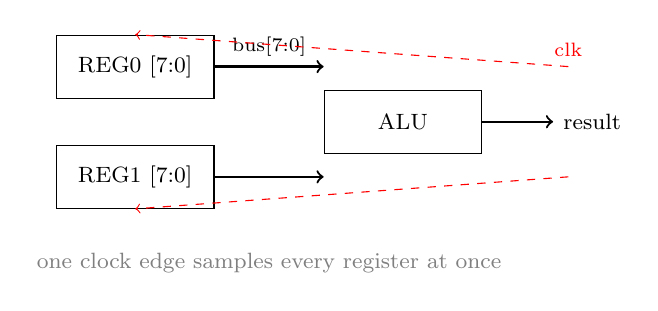
\begin{tikzpicture}[font=\footnotesize, reg/.style={draw, minimum width=2.0cm, minimum height=0.8cm}]
\node[reg] (r0) at (0,0) {REG0 [7:0]};
\node[reg] (r1) at (0,-1.4) {REG1 [7:0]};
\node[reg] (alu) at (3.4,-0.7) {ALU};
\draw[->, thick] (r0.east) -- node[above, font=\scriptsize] {bus[7:0]} (alu.west |- r0.east);
\draw[->, thick] (r1.east) -- (alu.west |- r1.east);
\draw[->, thick] (alu.east) -- ++(0.9,0) node[right] {result};
\draw[->, dashed, red] (5.5,0) node[above, font=\scriptsize] {clk} -- (r0.north);
\draw[->, dashed, red] (5.5,-1.4) -- (r1.south);
\node[gray] at (1.7,-2.5) {one clock edge samples every register at once};
\end{tikzpicture}

\caption{Registers around an ALU. Notice the same \texttt{clk} fans
out to every register — one edge, every value sampled simultaneously;
between edges the combinational ALU settles.}
\label{fig:register}
\end{figure}

\section{Counters}
\label{sec:counters}

A \emph{counter}\index{counter} is a register that adds 1 per edge.
Ripple counters chain toggle flip-flops (Figure~\ref{fig:counter});
synchronous counters compute \texttt{q+1} in parallel — the useful
ones add \texttt{en} (only count when told) and a terminal-count flag.

\begin{figure}[htbp]
\centering
% counter structure
\begin{tikzpicture}[font=\footnotesize, cell/.style={draw, minimum width=1.3cm, minimum height=0.8cm}]
\node[cell] (t0) at (0,0) {TFF0};
\node[cell] (t1) at (1.9,0) {TFF1};
\node[cell] (t2) at (3.8,0) {TFF2};
\node[cell] (t3) at (5.7,0) {TFF3};
\draw[->, red, thick] (-1,0) node[left] {clk} -- (t0.west);
\draw[->, thick] (t0.east) -- node[above, font=\scriptsize] {$q_0$} (t1.west);
\draw[->, thick] (t1.east) -- node[above, font=\scriptsize] {$q_1$} (t2.west);
\draw[->, thick] (t2.east) -- node[above, font=\scriptsize] {$q_2$} (t3.west);
\draw[->, thick] (t3.east) -- ++(0.5,0) node[right, font=\scriptsize] {$q_3$};
\draw[->, ink] (0,-0.8) node[left] {en} -- ++(0.4,0) |- (t0.south);
\node[gray] at (2.8,-1.7) {each T flip-flop toggles only when all lower bits are 1};
\end{tikzpicture}

\caption{Counter structure. Notice each stage toggles only when every
lower bit is 1 — counting is carry-propagation made visible.}
\label{fig:counter}
\end{figure}

\begin{lstlisting}[caption={\ttfamily code/ch10\_counter.v ---
enable + terminal count.},label={lst:counter},abovecaptionskip=0pt]
module counter(clk, en, q, tc);
  input clk, en;
  output reg [3:0] q = 0;
  output tc;
  assign tc = (q == 4'd15) & en;
  always @(posedge clk)
    if (en) q <= q + 1;
endmodule
\end{lstlisting}

\begin{lstlisting}[caption={Real run tail --- rollover at 15 with
\texttt{tc} asserted, counting resumes from 0.},abovecaptionskip=0pt]
t=155 en=1 | q=15 tc=1
t=165 en=1 | q= 0 tc=0
t=175 en=1 | q= 1 tc=0
\end{lstlisting}

\section{Worked example 2: a 1 Hz tick from 27 MHz}
\label{sec:we-tick}

\textbf{Strategy.} The Tang Nano 9K board's oscillator runs at 27 MHz;
blinking an LED at 1 Hz needs a prescaler that counts
$27\,000\,000$ cycles, then toggles — a counter with a terminal count
wired to an output flip.

\textbf{Solution.} $\log_2(27{\times}10^6)\approx 24.7$, so a 25-bit
counter suffices. Count to $13\,500\,000$, reset, toggle the blink:
$13.5{\times}10^6$ ticks per half-second. In Verilog the whole prescaler
is one \texttt{if} inside the \texttt{always} block plus an output flip —
the same \texttt{counter} pattern at scale. The honest check: the LED
pin needs only the toggle — the count is internal state, exactly what
registers are for.

\section{Finite state machines}
\label{sec:fsm}

An \emph{FSM}\index{finite state machine} is states + edges + outputs:
a register holding the state, combinational next-state logic, and
output logic. \emph{Moore}\index{Moore machine} outputs depend on state
only; \emph{Mealy}\index{Mealy machine} outputs also take the inputs
directly (Figure~\ref{fig:mealy_moore}). The disciplined three-block
style — one \texttt{always} per job — keeps the machine readable and
the synthesizer honest.

\begin{figure}[htbp]
\centering
% Mealy vs Moore templates
\begin{tikzpicture}[font=\footnotesize,
  box/.style={draw, rounded corners=2pt, minimum width=2.4cm, minimum height=1.1cm, align=center}]
\node[box] (regm) at (0,2.4) {state\\ register};
\node[box] (nxtm) at (3.8,2.4) {next-state\\ logic};
\node[box] (outm) at (3.8,0.4) {output logic\\ Moore: f(state)};
\draw[->, thick] (-1.8,2.4) node[left] {in} -- (nxtm.west);
\draw[->, thick] (regm.east) -- (nxtm.west);
\draw[->, thick] (regm.east) |- (outm.west);
\draw[->, thick] (outm.east) -- ++(0.8,0) node[right] {out};
\draw[->, thick] (nxtm.south) |- (regm.north);
% mealy path
\draw[->, thick, accent, dashed] (-1.8,2.4) ++(0,-0.15) .. controls (1,1.1) .. (outm.west)
  node[midway, above, font=\scriptsize, accent] {Mealy: inputs reach output directly};
\end{tikzpicture}

\caption{Moore vs Mealy. Notice the dashed path: only Mealy lets inputs
reach the output within the same cycle — one edge faster, one glitch
path wider.}
\label{fig:mealy_moore}
\end{figure}

\section{Worked example 3: the traffic-light FSM, end to end}
\label{sec:we-traffic}

\textbf{Strategy.} State diagram first (Figure~\ref{fig:fsm}), then an
encoding, then the three-block Verilog, then the simulator prints the
cycle for us to check against the diagram.

\textbf{Solution.} Four states — NS green, NS yellow, EW green, EW
yellow — each transition on a timer:

\begin{figure}[htbp]
\centering
% traffic FSM state diagram (Moore)
\begin{tikzpicture}[font=\footnotesize, state/.style={draw, circle, minimum size=1.9cm, align=center, inner sep=1pt}]
\node[state] (g1) at (0,0) {NS\_G\\ \scriptsize NS=grn, EW=red};
\node[state] (y1) at (3.4,0) {NS\_Y\\ \scriptsize NS=ylw, EW=red};
\node[state] (g2) at (3.4,-3.0) {EW\_G\\ \scriptsize EW=grn, NS=red};
\node[state] (y2) at (0,-3.0) {EW\_Y\\ \scriptsize EW=ylw, NS=red};
\draw[->, thick] (g1) -- node[above] {timer} (y1);
\draw[->, thick] (y1) -- node[right] {timer} (g2);
\draw[->, thick] (g2) -- node[below] {timer} (y2);
\draw[->, thick] (y2) -- node[left] {timer} (g1);
\draw[->, dashed, ink] (-1.4,1.4) node[left] {rst} -- (g1.north west);
\end{tikzpicture}

\caption{The traffic machine. Notice outputs ride \emph{inside} the
states (Moore): NS is green only in \texttt{NS\_G}, full stop.}
\label{fig:fsm}
\end{figure}

\begin{lstlisting}[caption={\ttfamily code/ch10\_traffic\_fsm.v ---
always-three-block style.},label={lst:fsm},abovecaptionskip=0pt]
module traffic_fsm(clk, rst, ns, ew);
  input clk, rst;
  output reg [1:0] ns, ew;
  localparam NS_G=2'd0, NS_Y=2'd1, EW_G=2'd2, EW_Y=2'd3;
  reg [1:0] state = NS_G, nxt;
  always @(*) begin
    case (state)
      NS_G: nxt = NS_Y;  NS_Y: nxt = EW_G;
      EW_G: nxt = EW_Y;  EW_Y: nxt = NS_G;
      default: nxt = NS_G;
    endcase
  end
  always @(posedge clk) state <= rst ? NS_G : nxt;
  always @(*) begin
    ns = (state==NS_G) ? 2'b00 : (state==NS_Y) ? 2'b01 : 2'b10;
    ew = (state==EW_G) ? 2'b00 : (state==EW_Y) ? 2'b01 : 2'b10;
  end
endmodule
\end{lstlisting}

\begin{lstlisting}[caption={The real full-cycle trace --- GRN
(\texttt{00})$\to$YEL (\texttt{01}) around the loop, EW red
(\texttt{10}) throughout the NS phase.},abovecaptionskip=0pt]
t= 15 rst=0 state=0 | NS=00 EW=10
t= 25 rst=0 state=1 | NS=01 EW=10
t= 35 rst=0 state=2 | NS=10 EW=00
t= 45 rst=0 state=3 | NS=10 EW=01
t= 55 rst=0 state=0 | NS=00 EW=10
\end{lstlisting}

The printed cycle matches the diagram edge-for-edge: NS goes green,
yellow, then EW green, yellow, and back — Moore outputs change only
when the state does.

\begin{exercise}[medium]
Extend the machine with a pedestrian-wait state entered from
\texttt{NS\_G} only when a button input is high. Which block changes —
next-state, register, or output?
\end{exercise}


\section{Worked example 4: Mealy answers a cycle early}
\label{sec:we-mealy}

\textbf{Strategy.} Give the same rising edge to a Moore detector and a
Mealy detector and watch the outputs disagree by exactly one cycle —
the price and prize of reading inputs at the output.

\textbf{Solution.}
\begin{lstlisting}[caption={\ttfamily code/ch10\_mm\_tb.v run ---
\texttt{mealy=1} at t=15, the cycle the edge lands;
\texttt{moore=1} waits for t=25.},abovecaptionskip=0pt]
t=  5 x=0 | mealy=0 moore=0
t= 15 x=1 | mealy=1 moore=0
t= 25 x=1 | mealy=0 moore=1
t= 35 x=0 | mealy=0 moore=1
\end{lstlisting}

Mealy's output is combinational on the input, so it fires \emph{in} the
edge's cycle — one cycle faster, and one glitch-path wider (a mid-cycle
wiggle on \texttt{x} would reach \texttt{yme} too). Moore's rides the
state, always a registered answer. Rule of thumb: outputs that must be
clean (LED, motor, write-enable) go Moore; outputs that must be quick
(requests, acknowledges) can pay the Mealy price.

\section{Worked example 5: the ``101'' detector, end to end}
\label{sec:we-seq101}

\textbf{Strategy.} The second classic FSM: detect \texttt{101} on a
serial input \emph{with overlap} (a found ``1'' may start the next
pattern). Four states, then let the sim find both hits in
\texttt{11010110}.

\textbf{Solution.}
\begin{lstlisting}[caption={\ttfamily code/ch10\_seq101.v --- the
overlap lives in \texttt{FOUND}'s edges.},label={lst:seq101},abovecaptionskip=0pt]
module seq101(clk, x, hit);
  input clk, x; output reg hit;
  localparam IDLE=0, GOT1=1, GOT10=2, FOUND=3;
  reg [1:0] st = IDLE, nx;
  always @(*) case (st)
    IDLE:  nx = x ? GOT1 : IDLE;
    GOT1:  nx = x ? GOT1 : GOT10;
    GOT10: nx = x ? FOUND : IDLE;
    FOUND: nx = x ? GOT1 : GOT10;   // overlap: the 1 restarts
    default: nx = IDLE;
  endcase
  always @(posedge clk) st <= nx;
  always @(*) hit = (st == FOUND);
endmodule
\end{lstlisting}

\begin{lstlisting}[caption={Real run over \texttt{11010110} --- hits at
t=45 and t=65, the second riding the first's last bit.},abovecaptionskip=0pt]
t= 35 x=1 state=2 hit=0
t= 45 x=0 state=3 hit=1
t= 55 x=1 state=2 hit=0
t= 65 x=1 state=3 hit=1
t= 75 x=0 state=1 hit=0
\end{lstlisting}

The overlap is the \texttt{FOUND} row: on \texttt{x=1} we go to
\texttt{GOT1}, not \texttt{IDLE} — that 1 was both the end of one
pattern and the start of the next. One line of the transition table
carries the whole ``with overlap'' requirement.

\section{Metastability and the two-flop rule}
\label{sec:meta}

One honest paragraph: a flip-flop whose input changes exactly at the
edge does not pick 0 or 1 — it can sit \emph{between} them, and may
stay undecided for an unbounded (but exponentially unlikely) time.
That \emph{metastability}\index{metastability} is physics, not a bug.
The defense is Figure~\ref{fig:sync}: run every asynchronous input
through \emph{two} flops — the first absorbs the rare bad sample, the
second sees only settled logic. \textbf{Never clock a button into
logic without the synchroniser}; every switch in later chapters goes
through this shape.

\begin{figure}[htbp]
\centering
% two-flop synchroniser
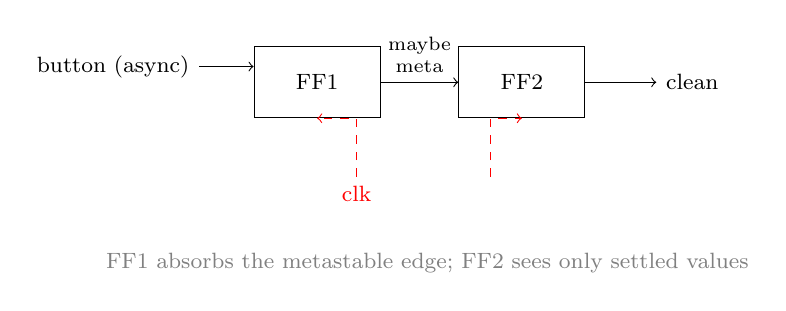
\begin{tikzpicture}[font=\footnotesize, cell/.style={draw, minimum width=1.6cm, minimum height=0.9cm}]
\node[cell] (f1) at (0,0) {FF1};
\node[cell] (f2) at (2.6,0) {FF2};
\draw[->] (-1.5,0.2) node[left] {button (async)} -- (f1.west |- 0,0.2);
\draw[->] (f1.east) -- node[above, font=\scriptsize, align=center] {maybe\\meta} (f2.west);
\draw[->] (f2.east) -- ++(0.9,0) node[right] {clean};
\draw[->, dashed, red] (0.5,-1.2) node[below] {clk} |- (f1.south);
\draw[->, dashed, red] (2.2,-1.2) |- (f2.south);
\node[gray] at (1.4,-2.3) {FF1 absorbs the metastable edge; FF2 sees only settled values};
\end{tikzpicture}

\caption{The two-flop synchroniser. Notice what is \emph{not} there:
no guarantee FF1 settles — only that FF2's input is one whole cycle
older, which settles the probability to negligible.}
\label{fig:sync}
\end{figure}

\section{Common mistakes}
\label{sec:mistakes}

\begin{itemize}
\item \textbf{Latch vs flip-flop confusion}: \texttt{@(*)} on
everything infers transparency and follows glitches — default to
\texttt{posedge} always.
\item \textbf{Incomplete sensitivity lists}: a \texttt{case} without
\texttt{default} leaves the output undriven on unlisted states and
invents a latch you never drew.
\item \textbf{Unreachable states}: an encoding wider than needed
leaves ghost states; route every default back somewhere real.
\item \textbf{Blocking vs nonblocking}: in clocked blocks use
\texttt{<=}; mixing is the classic silent-race source.
\item \textbf{Async inputs to logic}: skipping the two-flop
synchroniser on a button works 99.9\% of the time — and fails on the
demo day.
\end{itemize}

\section{Exercises}
\label{sec:exercises}

\begin{exercise}[easy]
Level vs edge: name the behavior each device exhibits and the Verilog
edge keyword for each.
\end{exercise}
\begin{exercise}[easy]
A 3-bit counter starting at 5: what are the next four counts?
\end{exercise}
\begin{exercise}[easy]
Which block of the three holds memory? Which two are pure combination?
\end{exercise}
\begin{exercise}[easy]
Why does Moore timing lag Mealy by up to a cycle?
\end{exercise}
\begin{exercise}[medium]
Pattern detector: FSM over bits detecting \texttt{101} with overlap.
Draw the states.
\end{exercise}
\begin{exercise}[medium]
Gray counter: why is Gray encoding safer for cross-domain sampling of
a count?
\end{exercise}
\begin{exercise}[medium]
The forgotten \texttt{else}: \texttt{if (en) q <= d;} inside
\texttt{@(*)} — what does the synthesizer build and why is it wrong?
\end{exercise}
\begin{exercise}[medium]
Prescaler: give the count value and bit width to get 10 Hz from 27 MHz.
\end{exercise}
\begin{exercise}[hard]
(Implement) Write \texttt{traffic\_tb} that asserts the exact state
cycle and count a violation; then add a walk-light state.
\end{exercise}
\begin{exercise}[hard]
A vending machine takes only 5- and 10-rupiah coins, dispenses at 15:
draw the FSM, encode it, and argue Moore vs Mealy.
\end{exercise}

\begin{exercise}[easy]
An SR latch with NOR gates: which inputs set, reset, and hold — and what
forbidden input pair breaks the abstraction?
\end{exercise}
\begin{exercise}[medium]
Register file: sketch two 8-bit registers and one shared bus; who decides
which register drives the bus, and what gate shape does it?
\end{exercise}
\begin{exercise}[medium]
Latency count: in the mm\_tb run, how many clock cycles separate the
first \texttt{mealy=1} from the last \texttt{moore=1}? Explain both.
\end{exercise}
\begin{exercise}[medium]
One-hot vs binary: our traffic machine used 2 bits for 4 states. Give
the one-hot encoding, its gate-count intuition, and when it wins.
\end{exercise}
\begin{exercise}[medium]
Serial adder: two numbers arrive one bit-pair per cycle. Draw the 2-state
FSM that outputs their sum (hint: one bit of state is a carry register —
you already built the combinational part in ch9).
\end{exercise}
\begin{exercise}[hard]
Design a debounced-button FSM: button $\to$ two-flop sync $\to$
edge-detect $\to$ one clean pulse per press, however long the press.
State the states.
\end{exercise}

\section{Summary}
\label{sec:summary}

\begin{center}\small
\begin{tabular}{@{}p{0.30\linewidth}p{0.62\linewidth}@{}}
\toprule
\textbf{Idea} & \textbf{One-line version} \\ \midrule
Latch & Transparent window — follows inputs while enabled. \\
Flip-flop & Photograph at the edge — the heartbeat's shutter. \\
Setup/hold & The edge contract; Book 7 does the math. \\
Register/bus & Edge-sampled row + the wires that feed it. \\
Counter & A register that adds 1 — \texttt{en} makes it a prescaler. \\
FSM (3 blocks) & State reg + next-state + output; never mix them. \\
Moore vs Mealy & State-only vs input-to-output path (1 cycle). \\
Metastability & Physics of the edge; sync it with two flops, always. \\
\bottomrule
\end{tabular}
\end{center}


\section*{Further reading}
\begin{itemize}
\item Harris \& Harris, \emph{Digital Design and Computer Architecture},
2nd ed., ch.\ 3 --- the reference for latch/FF discipline and FSM style;
free companion materials at \url{pages.hmc.edu/harris/ddca/}
(undergraduate level; the chapter's primary source~\cite{ddca}).
\item Kuphaldt, \emph{All About Circuits} Vol.\ IV (Digital),
sequential chapters --- alternative prose walk-through of the same
ladder; free textbook~\cite{aacvol4}.
\item MIT OCW \emph{6.004 Computation Structures} (2017) ---
university-level sequential logic lectures and labs, course page on
\url{ocw.mit.edu}
(undergraduate level; the academic version of this chapter).
\item Nisan \& Schocken, \emph{nand2tetris.org/course} project 3
(Memory) --- build the same registers bottom-up from DFFs in their HDL
(intro level; a second implementation of the same ideas).
\item HDLBits, \texttt{hdlbits.01xz.net} --- the Circuits/Sequential
problem set: small self-checking FSM drills named in the exercises
(practice engine, free).
\item \emph{fpga4fun.com} --- short real FPGA projects that consume
exactly these primitives (project ideas, intermediate).
\end{itemize}

\begin{rulebox}[Watch instead]
\begin{itemize}
\item \emph{Building an 8-bit breadboard computer} (full playlist),
Ben Eater, $\sim$20 videos --- the register/counter/FSM concepts here
built physically on breadboards; matches \S\ref{sec:feedback},
\S\ref{sec:setup}, \S\ref{sec:counters}. Accessed 2026-10-11.
\item \emph{D flip-flop} (single video), Ben Eater, $\sim$15 min ---
the DFF built from gates in front of you; matches
\S\ref{sec:feedback}--\S\ref{sec:we-latch}. Accessed 2026-10-11.
\end{itemize}
\end{rulebox}

\section*{Notes}
\begin{enumerate}
\item Harris \& Harris, \emph{Digital Design and Computer Architecture},
ch.\ 3 — latches, flops, FSM style~\cite{ddca}.
\item \emph{All About Circuits}, Vol.~IV: Digital — sequential
building blocks~\cite{aacvol4}.
\item HDLBits problem sets — the FSM drills named in the
exercises~\cite{hdlbits}.
\end{enumerate}

\section*{Hints and answers}
\begin{description}
\item[Trace (medium)] FF samples $d$ at t=5 (=1), 15 (=0), 25 (=1);
the latch passed the t=16 value mid-window, the FF waited to t=25.
\item[Pedestrian (medium)] Next-state logic + encoding only; outputs
ride on the states (Moore).
\item[Level/edge (easy)] Latch: level, \texttt{@(*)}; FF: edge,
\texttt{posedge clk}.
\item[3-bit count (easy)] 5,6,7,0,1.
\item[Blocks (easy)] The state register; next-state and output are
combinational.
\item[Moore lag (easy)] Outputs settle only after the state advances.
\item[101 detector (medium)] 4 states (none/1/10/101); on completion
input 0 sends you back for overlap.
\item[Gray (medium)] Only one bit flips per step — an async sample
can be off by at most one count.
\item[Missing else (medium)] Unassigned paths infer a latch holding
\texttt{q} — an invisible memory you never drew.
\item[10 Hz prescaler (medium)] $1.35{\times}10^6$ ticks per
half-period, 21 bits.
\item[Walk light (hard)] One more state + a \texttt{walk} input; the
tb's cycle assertion catches any skipped state.
\item[Vending (hard)] 4 states (0/5/10/dispense); Moore keeps the
dispense output glitch-free.
\item[SR latch (easy)] S=1 sets, R=1 resets, both 0 holds; S=R=1 is the
forbidden pair (output depends on release order).
\item[Register file (medium)] An enable line per register picks the
driver; each output goes through a mux or tri-state buffer.
\item[Latency count (medium)] t=15 to t=35: two edges — Mealy fires in
the sample's own cycle, Moore only after the state advances.
\item[One-hot (medium)] 4 bits, one hot per state; next-state logic is
one AND-OR row per destination — wins when speed beats area and $n$
is small.
\item[Serial adder (medium)] 2 states C=0/C=1 (the carry); each cycle
outputs $a_i\oplus b_i\oplus C$ and stores the new carry.
\item[Debounce (hard)] States idle/pressed/wait-release + a settling
counter; pulse out on the synced edge only.
\end{description}
